\documentclass[a4paper,11pt]{article}

\usepackage{wrapfig}
\usepackage{amsmath}
\usepackage{pgfplots}
\usepackage{enumerate}
\usepackage{cancel}
\usepackage{chngcntr}
\usepackage{graphicx}
\usepackage[most]{tcolorbox} % для управления цветом
%Russian-specific packages
%--------------------------------------
\usepackage[T2A]{fontenc}
\usepackage[utf8]{inputenc}
\usepackage[russian, english]{babel}
%--------------------------------------

\graphicspath{ {./img/} }

%Для выделения блока текста в рамку
\definecolor{block-gray}{gray}{0.95} % уровень прозрачности (1 - максимум)
\newtcolorbox{importantblock}{colback=block-gray,grow to right by=-10mm,grow to left by=-10mm,
boxrule=0pt,boxsep=0pt,breakable} % настройки области с изменённым фоном

\definecolor{lemonchiffon}{rgb}{1.0, 0.98, 0.8}
\newtcolorbox{mainblock}{colback=lemonchiffon,grow to right by=-10mm,grow to left by=-10mm,
boxrule=0pt,boxsep=0pt,breakable} % настройки области с изменённым фоном

\makeatletter
\newcommand{\settag}[1]{
  \tag*{(#1)\qquad}
  \edef\@currentlabel{\theequation#1}}
\makeatother

\counterwithin*{equation}{subsection}

\title{23. Методы последовательных приближений и Ньютона для решения нелинейных уравнений и систем}
\author{Андрей Бареков \and Ярослав Пылаев \and По лекциям Устинова С.М.}
\date{\today}

\begin{document}
\maketitle
\newpage

\section{Одно нелинейное уравнение}
\subsection{Метод последовательных приближений}
\begin{equation}
  f(x) = 0.
  \label{eq:NonLinearEq}
\end{equation}
Эквивалентными преобразованиями приведем уравнение (\ref{eq:NonLinearEq}) к виду
\begin{equation}
  x = \varphi(x).
  \label{eq:NewNonLinearEq}
\end{equation}
Корень нелинейного уравнения
\begin{equation*}
  x^* = x_n + \varepsilon_n, \hspace{3mm} x^* = \varphi(x^*).
\end{equation*}
Вместо уравнения (\ref{eq:NewNonLinearEq}) решаем разностное уравнение
\begin{equation}
  x_{n+1} = \varphi(x_n).
\end{equation}
Оценим сходимость:
\begin{align*}
  \underline{\varepsilon_{n+1}} &= x^* - x_{n+1} = \varphi(x^*) - \varphi(x_n) = \varphi(x_n+\varepsilon_n) - \varphi(x_n) = \\
        &= \underbrace{\varphi(x_n) + \varepsilon_n\varphi^{'}(\eta)}_ {\text{разложили в ряд}} - \varphi(x_n) =  \underline{\varepsilon_n\varphi^{'}(\eta)}.
\end{align*}
Убывание погрешности гарантирует условие
\begin{equation*}
  \bigg| \varphi^{'}(\eta) \bigg| < 1. \settag{*}
\end{equation*}
\begin{importantblock}
  Искусство пользователя заключается в том, чтобы перейти от уравнения (\ref{eq:NonLinearEq}) к (\ref{eq:NewNonLinearEq}) так, чтобы выполнялось условие ($*$).
\end{importantblock}

\subsection{Метод Ньютона (\textit{касательных})}
\begin{equation}
  f(x) = 0.
  \label{eq:NonlinearEq}
\end{equation}
Подставим в уравнение (\ref{eq:NonLinearEq}) его корень $x^*=x_n+\varepsilon_n$ и разложим \\ в ряд по степени $\varepsilon_n$:
\begin{equation}
  0 = f(x^*) = f(x_n+\varepsilon_n) = f(x_n)+\varepsilon_nf^{'}(x_n)+\frac{\varepsilon_n^2}{2!}f^{''}(\eta),
\end{equation}
пренебрежем последним слагаемым и для $\varepsilon_n$ получим
\begin{equation*}
  \varepsilon_n = - \frac{f(x_n)}{f^{'}(x_n)}.
\end{equation*}
Тогда
\begin{equation}
  x_{n+1} = x_n - \frac{f(x_n)}{f^{'}(x_n)}.
\end{equation}

\begin{center}
  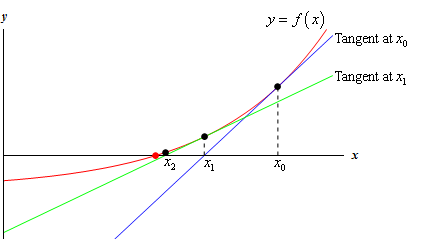
\includegraphics[scale=0.8]{img1.png}
\end{center}

\begin{align*}
  &P(x) = f(x_n) + f^{'}(x_n)(x-x_n) - \text{уравнение касательной}, \\
  &P(x) = 0, \Rightarrow \text{следующее приближение: } x_{n+1} = x_n - \frac{f(x_n)}{f^{'}(x_n)}.
\end{align*}

\subsubsection{Сходимость метода}
\begin{gather*}
  x^* = x^*, x_{n+1}+\varepsilon_{n+1} = x_n+\varepsilon_n, \\
  \varepsilon_{n+1} = \varepsilon_n + \frac{f(x_n)}{f^{'}(x_n)} = \frac{\overbrace{f(x_n) + \varepsilon_nf^{'}(x_n)}^{\text{см. ($2$)}}}{f^{'}(x_n)} =
  -\frac{f^{''}(\eta)}{2f^{'}(x_n)}\varepsilon_n^2.
\end{gather*}
Тогда если \[\bigg| \frac{f^{''}(\eta)}{2f^{'}(x_n)} \bigg| < C,\] где $C$ - константа, то
\begin{equation}
  \bigg| \varepsilon_{n+1} < \varepsilon_n^2 \bigg|,
\end{equation}
\begin{center}
  \small \textit{квадратичная скорость сходимости.}
\end{center}

\noindent Метод Ньютона \textit{очень быстро} сходится, но, конечно, \textit{если} сходится. Как правило он требует очень хорошего начального приближения.
Поэтому на практике его часто используют в паре, например, с методом бисекции, который как раз обеспечивает хорошее начальное приближение,
а затем уже метод Ньютона - квадратичную скорость сходимости. \\

\noindent Также на практике применяют \textit{модификации} метода Ньютона:
\begin{itemize}
  \item производная не пересчитывается \[x_{n+1} = x_n - \frac{f(x_n)}{f^{'}(x_0)}.\]
  \item метод с регулировкой шага \[x_{n+1} = x_n - \alpha\frac{f(x_n)}{f^{'}(x_n)}.\]
    Для расширения области сходимости первоначально $\alpha<1$, а при приближении к $0$ $\alpha=1$ и возвращается обычный вид метода.
\end{itemize}

\section{Система нелинейных уравнений}
\begin{align}
  f(x) = 0, && x \in R^N, \hspace{1mm}f \in R^n, && x = \begin{pmatrix} x^{(1)} \\ x^{(2)} \\ \dots \\ x^{(N)} \end{pmatrix}, &&
  f = \begin{pmatrix} f^{(1)} \\ f^{(2)} \\ \dots \\ f^{(N)} \end{pmatrix}.
\end{align}

\subsection{Метод последовательных приближений для решения систем уравнений}
Метод сохраняет свой вид и для систем уравнений
\begin{gather}
  f(x) = 0, \\
  x = \varphi(x), \\
  x_{n+1} = \varphi(x_n).
\end{gather}
Система ($1$) эквивалентными преобразованиями приводится к виду ($2$). Далее решаем систему разностных уравнений ($3$) пошаговым методом.\\

\noindent Для одного уравнения условие сходимости имеет вид
\begin{equation*}
  |\varphi^{'}(n)| < 1. \settag{*}
\end{equation*}
Для системы уравнений аналогичное условие сходимости  выглядит следующим образом:
\begin{gather*}
  \parallel\frac{\partial\varphi}{\partial x}\parallel < 1, \settag{**}.
\end{gather*}
\begin{align*}
  &\frac{\partial\varphi}{\partial x} \text{ - матрица Якоби}, \\
  &\frac{\partial\varphi}{\partial x} =
  \begin{pmatrix}
    \frac{\partial\varphi^{(1)}}{\partial x^{(1)}} & \frac{\partial\varphi^{(1)}}{\partial x^{(2)}} & \cdots & \frac{\partial\varphi^{(1)}}{\partial x^{(n)}} \\
    \hdotsfor{4} \\
    \frac{\partial\varphi^{(n)}}{\partial x^{(1)}} & \frac{\partial\varphi^{(n)}}{\partial x^{(2)}} & \cdots & \frac{\partial\varphi^{(n)}}{\partial x^{(n)}}
  \end{pmatrix}
\end{align*}
\begin{importantblock}
  Искусство пользователя заключается в том, чтобы привести систему ($1$) к виду ($2$) так, чтобы выполнялось условие ($**$).
\end{importantblock}

\subsection{Метод Ньютона для решения систем уравнений}
Применение метода Ньютона для систем уравнений проиллюстрируем на примере системы из двух уравнений.
\begin{equation}
  f(x) = 0,
\end{equation}
\begin{equation*}
  x^* = x_n + \varepsilon_n.
\end{equation*}
Введем обозначения:
\begin{align*}
  x^* = \begin{pmatrix} x_*^{(1)} \\ x_*^(2) \end{pmatrix}, && x_n = \begin{pmatrix} x_n^{(1)} \\ x_n^(2) \end{pmatrix}, &&
  \varepsilon_n = \begin{pmatrix} \varepsilon_n^{(1)} \\ \varepsilon_n^(2) \end{pmatrix}.
\end{align*}
Рассмотрим первое уравнение системы ($1$) и подставим в него точное решение
\begin{align*}
  0 &= f^{(1)}\bigg( x_*^{(1)}, x_*^{(2)} \bigg) = f^{(1)}\bigg( x_n^{(1)}+\varepsilon_n^{(1)}, x_n^{(2)}+\varepsilon_n^{(2)} \bigg) = \\
  &= \bigg[\text{раскладываем в ряд по $\varepsilon_n^{(1)}$ и $\varepsilon_n^{(2)}$ пренебрегая малыми второго порядка} \bigg] = \\
  &= f^{(1)}\bigg( x_n^{(1)}, x_n^{(2)} \bigg) + \frac{\partial f^{(1)}}{\partial x^{(1)}} \bigg( x_n^{(1)}, x_n^{(2)} \bigg)\varepsilon_n^{(1)} +
    \frac{\partial f^{(1)}}{\partial x^{(2)}} \bigg( x_n^{(1)}, x_n^{(2)} \bigg)\varepsilon_n^{(2)} + \cdots = 0.
\end{align*}
Получили
\begin{equation}
  \frac{\partial f^{(1)}}{\partial x^{(1)}} \bigg( x_n^{(1)}, x_n^{(2)} \bigg)\varepsilon_n^{(1)} +
    \frac{\partial f^{(1)}}{\partial x^{(2)}} \bigg( x_n^{(1)}, x_n^{(2)} \bigg)\varepsilon_n^{(2)} = -f^{(1)}\bigg( x_n^{(1)}, x_n^{(2)} \bigg).
\end{equation}
Аналогично и для второго уравнения
\begin{equation}
  \frac{\partial f^{(2)}}{\partial x^{(1)}} \bigg( x_n^{(1)}, x_n^{(2)} \bigg)\varepsilon_n^{(1)} +
    \frac{\partial f^{(2)}}{\partial x^{(2)}} \bigg( x_n^{(1)}, x_n^{(2)} \bigg)\varepsilon_n^{(2)} = -f^{(2)}\bigg( x_n^{(1)}, x_n^{(2)} \bigg).
\end{equation}
Эту систему уравнений можно записать в матричном виде:
\begin{equation}
  \boxed{
  \begin{cases}
    \frac{\partial f}{\partial x}(x_n)\varepsilon_n = -f(x_n), \\
    x_{n+1} = x_n+\varepsilon_n
  \end{cases}}
\end{equation}
\begin{center}
  \small метод Ньютона для систем уравнений, где $\frac{\partial f}{\partial x}$ - матрица Якоби.
\end{center}
На каждом шаге приходится решать систему линенейных алгебраических уравнений относительно вектора $\varepsilon_n$ (вспоминаем о подпрограммах $DECOMP$ и  $SOLVE$). \\

\noindent Формула ($4$) обладает всеми \textit{достоинствами} и \textit{недостатками} метода Ньютона для одного уравнения:
\begin{itemize}
  \item квадратичная скорость сходимости,
  \item требование хорошего начального приближения.
\end{itemize}

\subsubsection{Модификация метода Ньютона для решения систем уравнений}
\begin{equation*}
  \begin{cases}
    \frac{\partial f}{\partial x}(x_0)\varepsilon_n = -f(x_n), \\
    x_{n+1} = x_n+\varepsilon_n
  \end{cases}
  \settag{4*}
\end{equation*}
Матрица Якоби вычисляется \textit{однократно} в точке $x_0$, \textit{однократно} выполняется ее $LU$-разложение, и на последующих шагах используется только
программа $SOLVE$. Матрица вычисляется вновь, только если нарушается (замедляется) сходимость.

\end{document}
